In this section we present the essential theoretical background and context for this thesis. First introducing fundamental concepts in software engineering, the software development lifecycle (SDLC), continuous integration (CI), and the software project hosting platforms. The second part explores the rising role of GenAi/LLMs in software development practices.The third part showcases the evolution and state of APR and explores existing approaches.

\section{Software Engineering}

The following section introduces core concepts starting with the software development lifecycle,the importance of Continuous Integration (CI) in modern software development and the role of code hosting platforms.
\subsection{Software Development Lifecycle}

Engineering and developing software is complex process, consisting of multiple different tasks. For structuring this process software development lifecycle models have been introduced. These models evolve constantly to adapt to the changing needs of creating software. The most promising and widely used model today is the Agile Software Development Lifecycle \cite{rupareliaSoftwareDevelopmentLifecycle2010}.

The Agile lifecycle brings an iterative approach to development, focusing on collaboration, feedback and adaptivity. The Goal is frequent delivery of small functional features of software, allowing for continuous improvement and adaptation to changing requirements. Using frameworks like Scrum or Kanban, an Agile iteration can be applied in a development environment\cite{rupareliaSoftwareDevelopmentLifecycle2010}.

\begin{figure}[H]
    \centering
    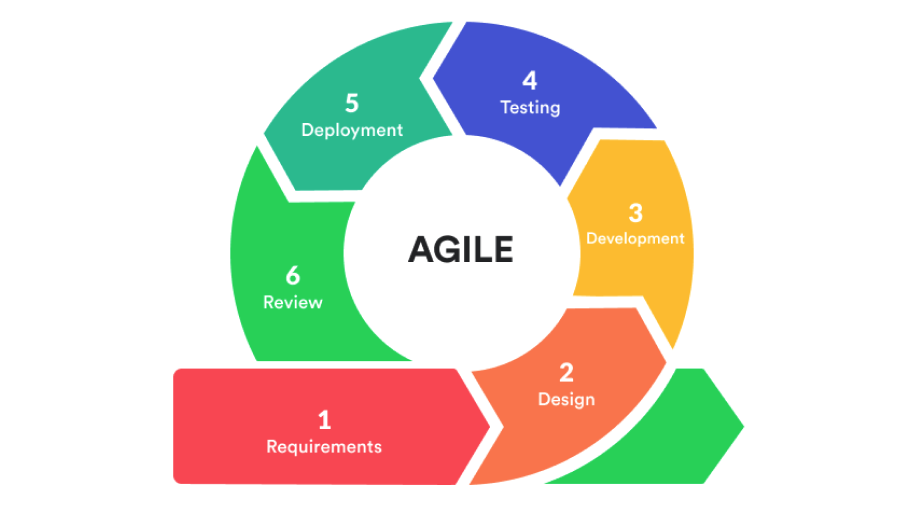
\includegraphics[width=1\textwidth]{images/agile-cycle.png}
    \caption{Agile Software Development Lifecycle}
    \label{fig:agile-cycle}
\end{figure}

An Agile Software Development Lifecycle iteration consists of 6 key stages like in Figure \ref{fig:agile-cycle} starting with planning phase where requirements for the iteration are gathered and prioritized. Secondly the design phase where the architecture and design of the feature is created. The third stage is where the actual development of the prioritized requirements takes place. After that the testing phase follows, where the software is tested for bugs and issues. The fifth stage is deployment, where the software is released to users. Finally, the changes are reviewed in a collaborative way.

When bugs arise during an iteration requirements can be reprioritized and the iteration can be adapted to fix these issues. This adaptivity is a key feature of Agile software development, allowing teams to respond quickly to changing requirements and issues but also slowing down delivery of planed features \cite{rupareliaSoftwareDevelopmentLifecycle2010}.

Modern software systems are moving towards lightly coupled microservice architectures, which results in more repositories which are smaller in scale tailored towards a specialized domain. This trend is driven by the need for flexibility, scalability, and faster development cycles. Smaller code repositories allow teams to work on specific components or services independently, reducing dependencies and enabling quicker iterations. This approach aligns with modern software development practices, such as microservices architecture and agile methodologies.
With this trend developers work on multiple projects at the same time, which can lead to more interruptions and context switching when problems arise and priorities shift.

\subsection{Continuous Integration}

For accelerating the delivery of software in an iteration continuous integration has become a standard in agile software development. The main objective of continuous integration is to accelerate phases 3 and 4 \cite{ugwuezeContinuousIntegrationDeployment2024}. CI allows for frequent code integration into a code repository. Automating steps like building and testing into the development resulting in rapid feedback right where the changes are committed in a shared repository. This supports critical aspects of agile software development, like fast delivery, fast feedback and enhanced collaboration \cite{ugwuezeContinuousIntegrationDeployment2024}.

\begin{figure}[H]
    \centering
    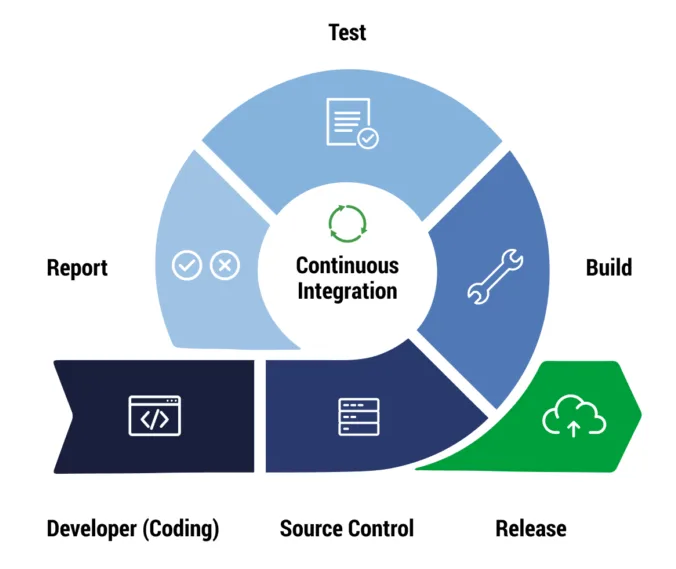
\includegraphics[width=1\textwidth]{images/ci-cycle.png}
    \caption{Continuous Integration Cycle}
    \label{fig:ci-cycle}
\end{figure}

Although CI bring a lot of potential to agile development it can also has drawbacks. Long build durations and high maintenance. %\cite{}

\subsection{Software Project Hosting Platforms} \label{subsection:Software Project Hosting Platforms}

Software projects live on platforms like Github or GitLab. With GitHub being the most popular and most used for open source %\cite{} 
These platforms offer tools and services for the entire software development lifecycle, including project hosting, version control, issue tracking, bug reporting, project management, backups, collaborative workflows, and documentation capabilities. \cite{abrahamssonAgileSoftwareDevelopment2017}

Github issues are a key feature of Github allowing for project scoped tracking of features, bugs, and tasks. Issues can be created, assigned, labeled, and commented on by everyone working on a codebase. This feature provides a structured way to manage and prioritize work within a project.

\begin{figure}[H]
    \centering
    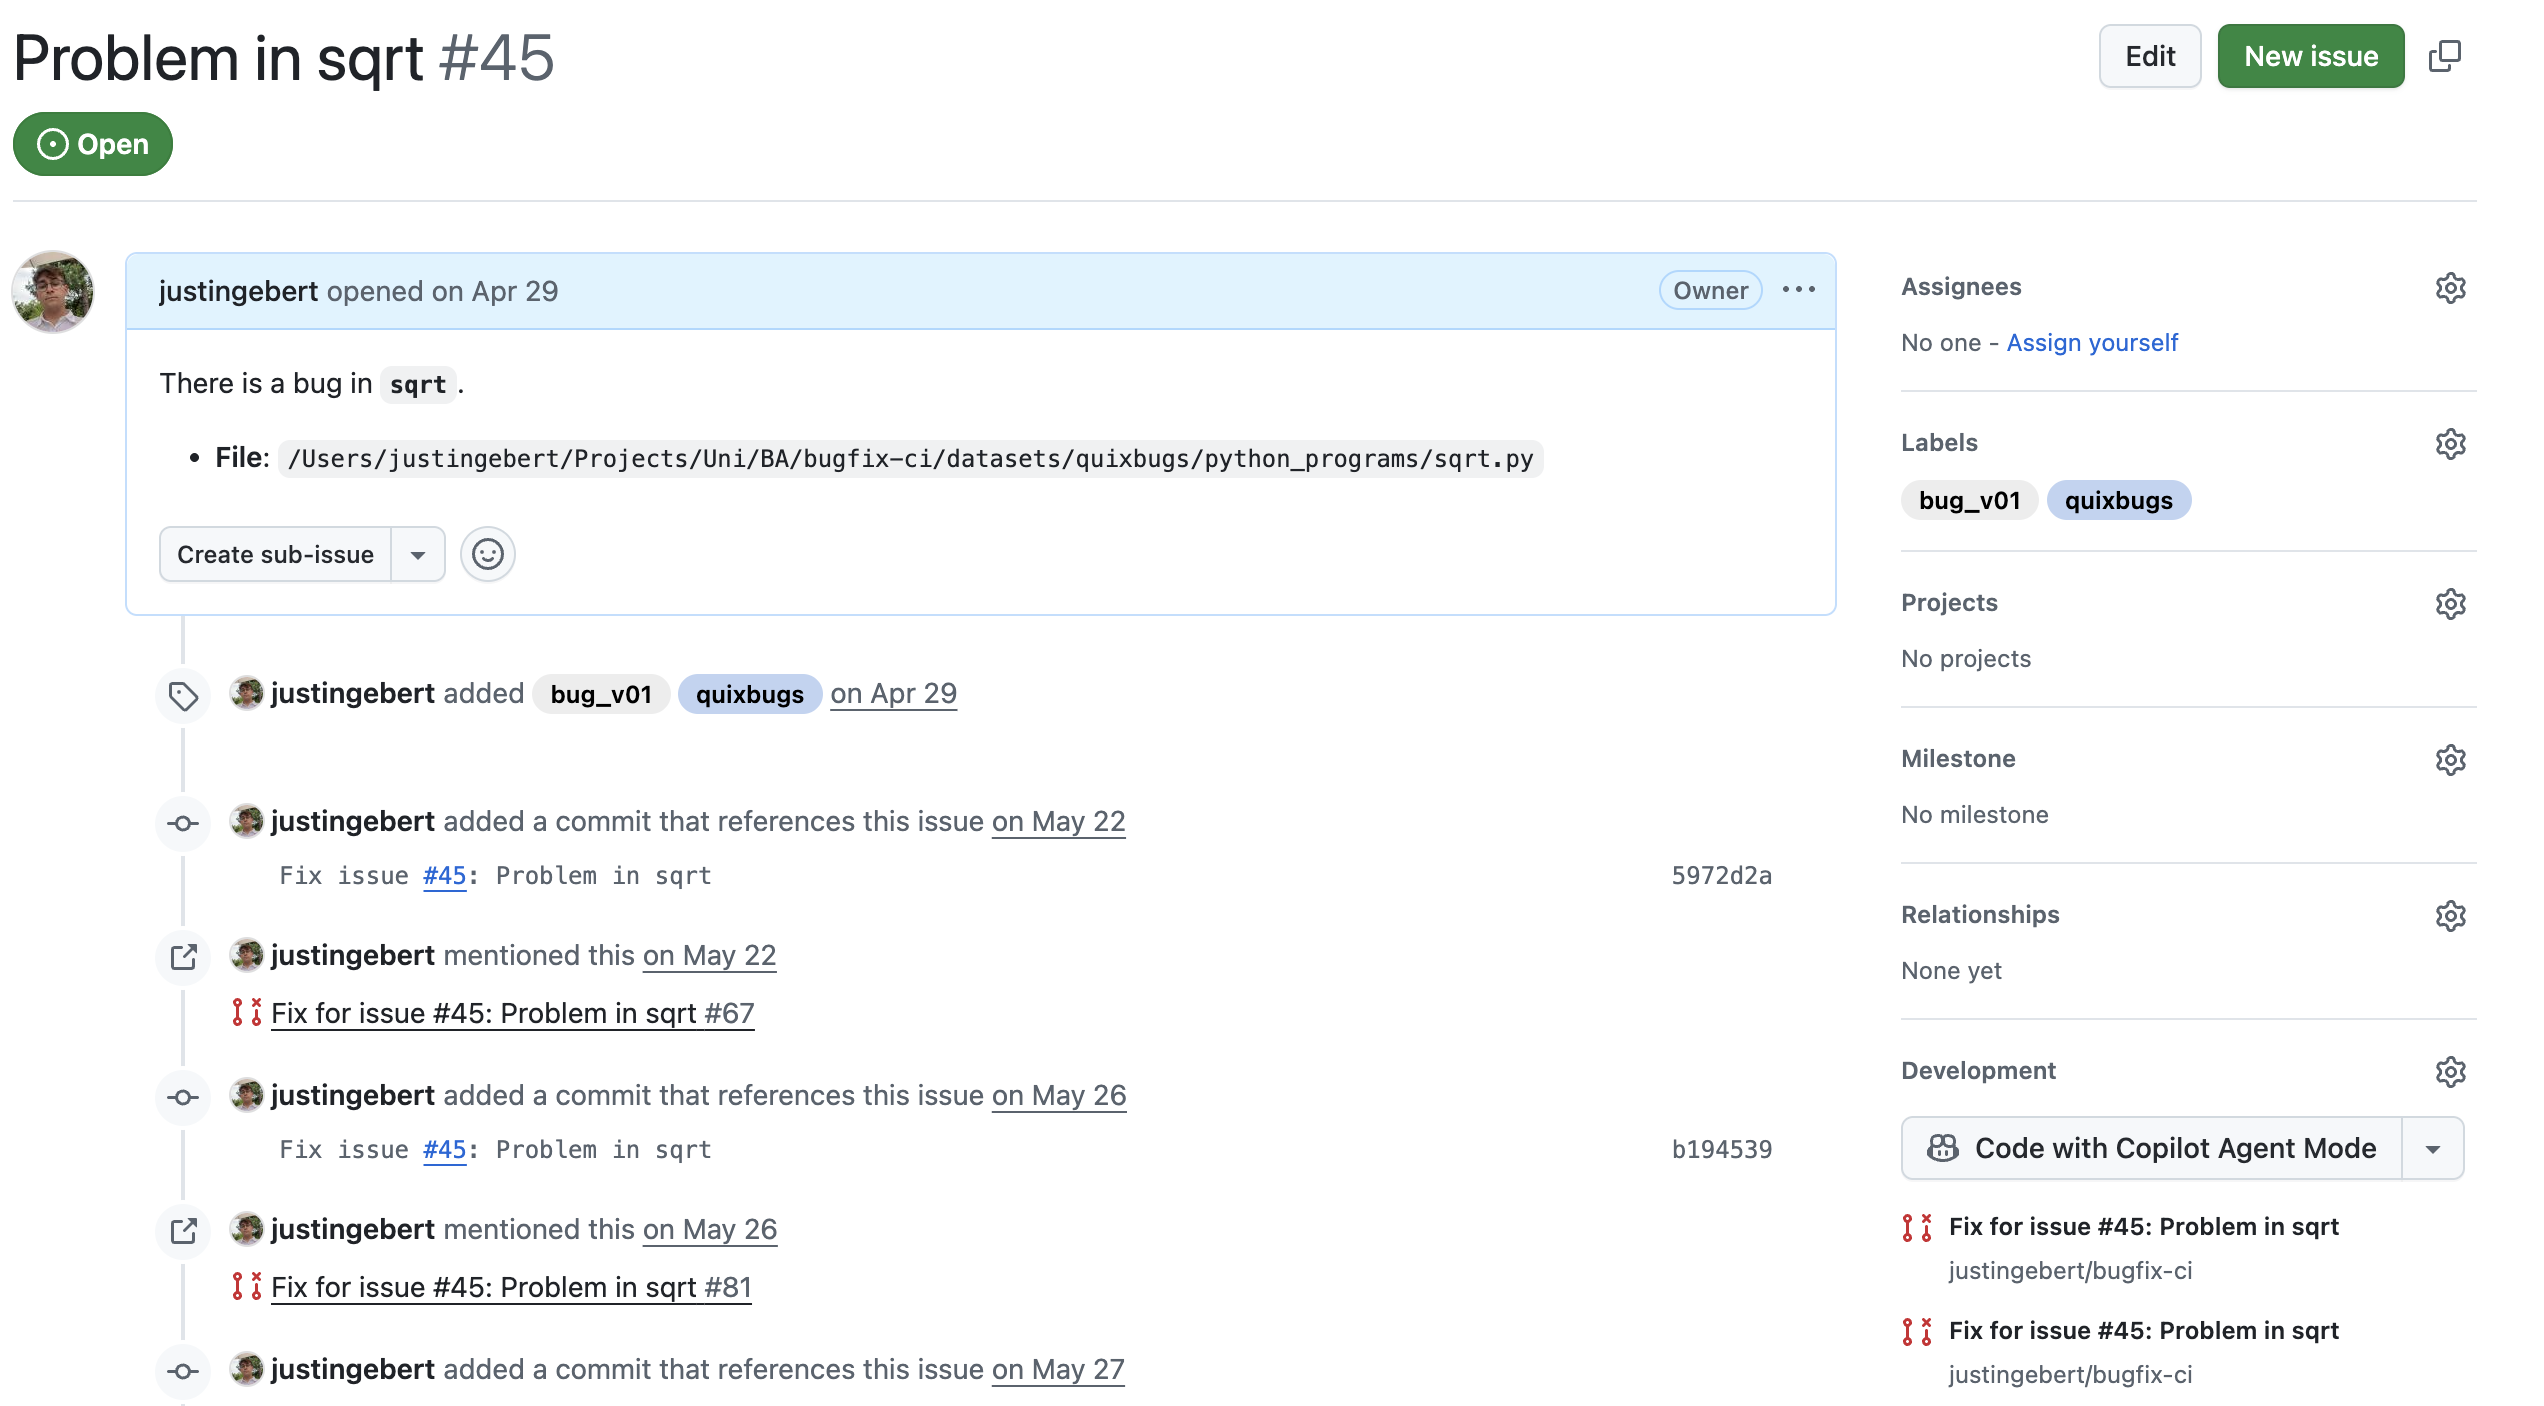
\includegraphics[width=1\textwidth]{images/github/GitHub Issue.png}
    \caption{Example of a GitHub Issue}
    \label{fig:gh-issue}
\end{figure}

For integrating and reviewing code into production GitHub provides Pull Requests. A Pull Request proposes changes to the codebase, providing an integrated review process to validate changes before they are integrated into the production codebase. Code changes are displayed in a diff format \footnote{TODO explain format} allowing reviewers to see and dig into the changes made.This process is essential for maintaining code quality and ensuring that changes are validated before being merged. %\cite{githubdoc}
Pull requests can be linked to Issues, allowing for easy tracking of changes related to specific tasks or bugs. %\cite{githubdoc}

GitHub also provides a manged solution (Github Actions) for integrating CI into a repositories by writing CI workflows in YAML files. Workflows can run as CI pipelines on runners hosted by GitHub or self hosted runners. A workflow consists of triggers and jobs, and steps. One or more events can trigger a workflow which executed one ore more jobs which are made up of one or more steps. \cite{Workflows} An example is shown in Figure \ref{fig:gh-workflow}. Workflow results and logs can be viewed from multiple points in the GitHub web UI, including the Actions tab, the Pull Request page, and the repository's main page. This integration provides a seamless experience for developers to monitor and manage their CI processes directly within their repositories.

\begin{figure}[H]
    \centering
    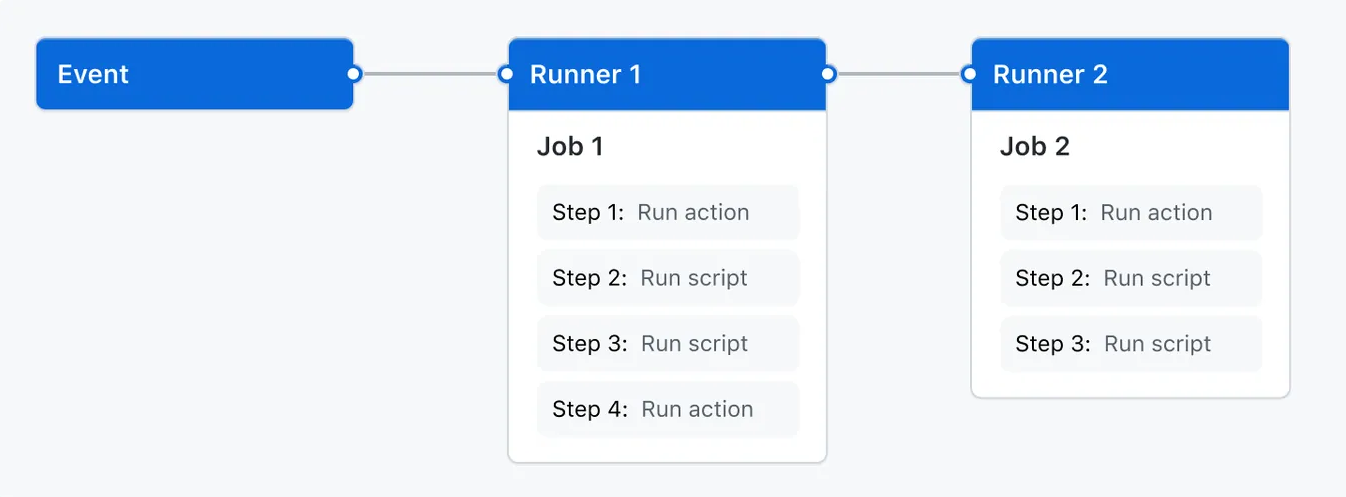
\includegraphics[width=1\textwidth]{images/overview-actions-simple.png}
    \caption{Simple Action}
    \label{fig:gh-workflow}
\end{figure}

\section{Generative AI in Software Development}

This section will cover the role of Generative AI in software development. First we will define Generative AI and Large Language Models (LLMs). The second part will focus on the impact of Generative AI on software development practices.
\subsection{Generative AI and Large Language Models}

Generative Artificial Intelligence (Gen AI) is subfield of artificial intelligence and refers to systems that can generate new content based on patterns learned from massive amounts of training data. Advanced machine learning techniques, particularly deep learning, enable these systems to generate text, images, or code, that resembles human-generated output.
In the field of natural language processing (NLP) was revolutionized by the Transformer architecture \cite{changSurveyEvaluationLarge2024}. It lays the ground work for Large Language Models which are specialized in text generation. Extensive training data results in Models billions of parameters, allows them to understand and generate human-like text in multiple natural languages and diverse programming languages. However this requires enormous computational resources during training and operation \cite{LLMsWhatsLarge}. A models parameter count has a direct impact on the model's performance, with larger models generally achieving better results in various NLP tasks but also demanding more computational resources %\cite{}. 
Despite modern LLMs showing promising results, they can still hallucinate incorrect or biased content. \cite{LLMsWhatsLarge}.

To archive a specific task using LLMs designing and providing specific input to the model to guide its output is called prompt engineering. This process is crucial for achieving desired results from LLMs, as the quality and specificity of the prompt directly influences the model's output. The input is constrained by a models context window, which is the maximum amount of text the model can process at once.

Popular Large Language Models are offered via APIs but providers like OpenAi, Anthropic and Google, or open source alternatives like X. Table \ref{table:llms} shows a selection of popular LLMs with their characteristics and performance on NLP benchmark X which evaluates X.
\begin{table}[ht]
    \centering
    \small
    \renewcommand{\arraystretch}{1.5}
    \begin{tabular*}{\textwidth}{@{\extracolsep{\fill}} p{3cm} | p{2cm} | p{2cm} | p{4cm} | p{2cm} @{}}
        \toprule
        \textbf{Model Name} & \textbf{Publisher} & \textbf{Parameters} & \textbf{Context Window Size} & \textbf{Cost per 1M} \\
        \midrule
        chatgpt & OpenAI & 175B & 1M & 1\$ \\ \hline
        \bottomrule
    \end{tabular*}
    \caption{Large Language Model Examples}
    \label{table:llms}
\end{table}


\subsection{Large Language Models in Software Development}

Large Language Models are reshaping software development by automating various tasks. They have billions of parameters and are pre-trained on massive codebases which results in extraordinary capabilities in this area \cite{chenUnveilingPitfallsUnderstanding2025}. Tools like Github Copilot, OpenAI Codex, and ChatGPT have become popular in the software development community, providing developers with AI-powered code suggestions and completions \cite{bhargavmallampatiRoleGenerativeAI2025}. These tools get applied in various stages of the software development lifecycle, including requirement engineering, code generation, debugging, refactoring, and testing \cite{houLargeLanguageModels2024, puvvadiCodingAgentsComprehensive2025,bhargavmallampatiRoleGenerativeAI2025}. By using LLMs to enhance the named tasks development cycle times can be reduced by up to 30 percent \cite{bhargavmallampatiRoleGenerativeAI2025,kalliamvakouResearchQuantifyingGitHub2022}. Furthermore these tools have positive impacts like improving developer satisfaction and reducing cognitive load \cite{kalliamvakouResearchQuantifyingGitHub2022}.

Although Generative AI gets adopted really quickly in many areas of software development this technology still faces limitations. LLMs have challenges working on tasks that are outside their scope of training or require specific domain knowledge \cite{houLargeLanguageModels2024}. Additionally LLMs have limited context windows, which can lead to challenges when working with large codebases or complex projects where context windows are too small for true contextual or requirements understanding \cite{bhargavmallampatiRoleGenerativeAI2025}. When generating code LLMs can produce incorrect or insecure code, which can lead to further bugs and vulnerabilities in the software \cite{houLargeLanguageModels2024, bhargavmallampatiRoleGenerativeAI2025}. Additionally when integrating LLMs into tools can be vulnerable to prompt injection, where unintended instructions are injected at some point and can also lead to production of harmful code \cite{liuPromptInjectionAttack2024}. Code generated by LLMs based on training data also raises questions about ownership, responsibility and intellectual property rights. \cite{sauvolaFutureSoftwareDevelopment2024, houLargeLanguageModels2024}.

Facing these challenges, different approaches have been developed. AI Agents, RAG or interactive approaches are prominent examples. These approaches aim to enhance the capabilities of LLMs by providing additional context, enabling multi-step reasoning, or allowing for interactive feedback loops during code generation and debugging \cite{houLargeLanguageModels2024, puvvadiCodingAgentsComprehensive2025}. Section \ref{subsection:evolution-apr} will go into more detail on these approaches.

Recently research is exploring solutions which integration LLMs into existing software development practices and workflows. \cite{puvvadiCodingAgentsComprehensive2025, dohmkeGitHubCopilotMeet2025, IntroducingCodex, sauvolaFutureSoftwareDevelopment2024}. This happens in tools and on platform where development happens and focuses on for example integrating AI/ML into CI/CD \cite{mohammedAIDrivenContinuousIntegration2024} or into code hosting platforms like GitHub \ref{subsection:Software Project Hosting Platforms}.

\section{Automated Program Repair}

Automated Program Repair (APR) is used to detect and repair bugs in code with minimal human intervention. \cite{zhangSurveyLearningbasedAutomated2024} APR systems are supposed to take over the process of fixing bugs, reducing load for developers and making time to focus on more relevant work. \cite{houLargeLanguageModels2024}

Using APR systems specific bugs can be fixed using a generated patch. Working patches are usually generated using a 3 stage approach: First localizing the bug. Then repairing the bug, in the end validation decides where the bug will be passed on \cite{zhangSurveyLearningbasedAutomated2024, baderGetafixLearningFix2019}. This approach is similar to the bug fixing process of a developer, where the bug is first identified, then fixed, and finally tested and reviewed to ensure the fix works as intended. An example of an APR system being applied at scale is Getafix, which is used at Meta to automatically fix common bugs in their production codebase \cite{baderGetafixLearningFix2019}.

The field of Automated program repair also greatly benefited of the rapid advancements in AI. With new research and benchmarks setting new standards in the field.\cite{puvvadiCodingAgentsComprehensive2025,houLargeLanguageModels2024}

In this section we will provide an overview of the evolution of APR, related work, and the current state of APR systems. Followed by a display of the most common APR benchmarks used in research.

\subsection{Evolution of Automated Program Repair} \label{subsection:evolution-apr}

We have seen multiple paradigm shifts in the field of Automated Program Repair (APR) over the years. This evolution of APR can be categorized into key stages, each marked by significant advancements in techniques and methodologies.

\textbf{Traditional Approaches:}

Traditional APR approaches typically rely on manual crafted rules and predefined pattern. \cite{liuMarsCodeAgentAInative2024, xiaAutomatedProgramRepair2023,yinThinkRepairSelfDirectedAutomated2024}. These methods are generally classified into three main categories: search based, constraint/semantic based, and template-based repair techniques.

\textbf{Search based repair} searches for the correct predefined patch in a large search space. \cite{liuMarsCodeAgentAInative2024, huCanGPTO1Kill2024,zhangPATCHEmpoweringLarge2025} A popular example is GenProg, which uses genetic algorithms to evolve patches by mutating existing code and selecting based on fitness determined by test cases \cite{legouesGenProgGenericMethod2012}.

\textbf{Semantics / constraint based repair} synthesizes patches using constraint solvers to based on semantic information of the program and tests. \cite{liuMarsCodeAgentAInative2024, mechtaevAngelixScalableMultiline2016} Angelix being a prominent example. \cite{mechtaevAngelixScalableMultiline2016}.

\textbf{Template based repair} relies on mined templates for transformations of known bugs. \cite{xiaAutomatedProgramRepair2023} Templates are mined from previous human produced bug fixes.\cite{xiaAutomatedProgramRepair2023, yinThinkRepairSelfDirectedAutomated2024}. Getafix being an example of an industrially deployed tool learning recurring fix pattern form past fixes \cite{baderGetafixLearningFix2019}

Traditional systems face significant limitations in scalability and adaptability. They struggle to generalize to new and unseen bugs, or to adapt to evolving codebases. Often requiring extensive computational resources and manual effort. \cite{puvvadiCodingAgentsComprehensive2025, xiaAutomatedProgramRepair2024}


\textbf{Learning based Approaches:}

Learning based APR introduced machine learning techniques to the field, improving the number and variety of bugs that can be fixed. Deep neural networks using bug fixing patterns from historical fixes as training data, learn how to generate patches to "translate" buggy code into correct code \cite{xiaAutomatedProgramRepair2023, tangLargeLanguageModels2024}. A prominent of a learning based APR system is CoCoNut \cite{lutellierCoCoNuTCombiningContextaware2020}, Recoder \cite{zhuSyntaxguidedEditDecoder2021}. Despite significant advancements these methods are limited by training data and struggle with unseen bugs. \cite{xiaLessTrainingMore2022}

\textbf{The emerge of LLM based APR:}

The explosive growth of LLMs has transformed the APR space. LLM based APR techniques have demonstrated significant improvements over all other state of the art techniques, benefitting from the coding knowledge \cite{hossainDeepDiveLarge2024}. For that reason LLMs lay the groundwork of a new APR paradigm \cite{chenUnveilingPitfallsUnderstanding2025, anandComprehensiveSurveyAIDriven2024}.

Different approaches leveraging LLMs have emerged and are being actively researched. These include:

\textbf{Retrieval-Augmented approaches} repair bugs with the help of retrieving relevant context during the repair process. For example code documentation stored in a vector database \cite{puvvadiCodingAgentsComprehensive2025}. This approach allows access to  external knowledge in the repair process, enhancing the LLM's ability to understand and fix bugs \cite{houLargeLanguageModels2024, yinThinkRepairSelfDirectedAutomated2024}.

\textbf{Interactive/Conversational approaches} make use of LLMs dialogue capabilities to provide patch validation with instant feedback. \cite{xiaAutomatedProgramRepair2024, huCanGPTO1Kill2024} This feedback is used to iterate and refine generated patches with the goal of archive better results. \cite{xiaAutomatedProgramRepair2024}

\textbf{Agent based system} improve bug localization and fixing by equipping LLMs with the ability to access external environments, operate tools (like file editors, terminals, web search engines), and make autonomous decisions. \cite{anandComprehensiveSurveyAIDriven2024, puvvadiCodingAgentsComprehensive2025, mengEmpiricalStudyLLMbased2024} Using multi-step reasoning these frameworks reconstruct the cognitive processes of developers using multiple specialized agents. \cite{rondonEvaluatingAgentbasedProgram2025,zhangPATCHEmpoweringLarge2025, leeUnifiedDebuggingApproach2024}. Examples include SWE-Agent \cite{yangSWEagentAgentComputerInterfaces2024}, FixAgent \cite{leeUnifiedDebuggingApproach2024}, MarsCodeAgent \cite{liuMarsCodeAgentAInative2024}, GitHub Copilot.

\textbf{Agentless systems} are a recent push towards more lightweight solutions, focusing on simplicity and efficiency. These approaches aim to reduce the complexity of APR systems by cutting complex multi-agent coordination and decision making, while maintaining effectiveness in bug fixing \cite{xiaAgentlessDemystifyingLLMbased2024,puvvadiCodingAgentsComprehensive2025}. This approach provides clear rails to the LLMs improving transparency of the bug fixing approach. Using 3 steps localization, repair, validation promising results with low costs have been achieved using this paradigm \cite{xiaAgentlessDemystifyingLLMbased2024, mengEmpiricalStudyLLMbased2024}.

Commonly used LLMs for the mentioned APR techniques include ChatGPT, Codex, CodeLlama, DeepSeek-Coder, and CodeT5 \cite{houLargeLanguageModels2024, yinThinkRepairSelfDirectedAutomated2024,anandComprehensiveSurveyAIDriven2024}.

Despite significant advancement state of the art APR system still face challenges and limitations. Existing system suffer from complexity with limited transparency and control over the bug fixing process.\cite{xiaAgentlessDemystifyingLLMbased2024,puvvadiCodingAgentsComprehensive2025, houLargeLanguageModels2024} The bug fixing process bugs takes a lot of computational resources and is time intensive making the program repair expensive \cite{sobaniaAnalysisAutomaticBug2023, puvvadiCodingAgentsComprehensive2025}. APR system are build and applied in controlled environments making APR unreachable for developers  since they cant be integrated into real world software development workflow and projects\cite{meemExploringExperiencesAutomated2024,puvvadiCodingAgentsComprehensive2025}

\subsection{APR benchmarks}
For standardizing evaluation in research of new APR approaches benchmarks have been developed. These benchmarks consist of a set of software bugs and issues, along with their corresponding fixes or tests, which can be used to evaluate the effectiveness of different APR techniques. \cite{anandComprehensiveSurveyAIDriven2024} They are essential for comparing the performance of different APR systems and understanding their strengths and weaknesses. \cite{puvvadiCodingAgentsComprehensive2025} APR benchmarks are available for different programming languages with popular ones being QuixBugs \cite{linQuixBugsMultilingualProgram2017}, Defects4J \cite{justDefects4JDatabaseExisting2014}, ManyBugs \cite{legouesManyBugsIntroClassBenchmarks2015} and SWE Bench \cite{jimenezSWEbenchCanLanguage2024}. \cite{wangSoftwareDevelopmentLife2025}

\begin{table}[ht]
    \centering
    \small
    \renewcommand{\arraystretch}{1.5}
    \begin{tabular*}{\textwidth}{@{\extracolsep{\fill}} p{2.5cm} | p{2cm} | p{1.5cm} | p{5cm} | p{4cm} @{}}
        \toprule
        \textbf{Model} & \textbf{Languages} & \textbf{Number of Bugs} & \textbf{Description} & \textbf{Difficulty} \\
        \midrule
        QuixBugs & Python, Java & 40 & small single line bugs  & Easy \\ \hline
        Defects4J & Java & 854 & real-world Java bugs & Medium \\ \hline
        ManyBugs & C & 185 & real-world C bugs & Medium \\ \hline
        SWE Bench & Python & 2294 & Real GitHub repository defects & Hard \\
        \hline
        SWE Bench Lite & Python & 300 & selected real GitHub defects & Hard \\
        \bottomrule
    \end{tabular*}
    \caption{Overview of APR Benchmarks}
    \label{table:benchmarks}
\end{table}